\documentclass[aspectratio=169]{beamer}
\usetheme{Madrid}
\usecolortheme{default}

\usepackage{graphicx}
\usepackage{amsmath}
\usepackage{amsfonts}
\usepackage{xcolor}
\usepackage{tikz}
\usepackage{pgfplots}

\definecolor{datacolor}{rgb}{0.2,0.4,0.8}
\definecolor{fitcolor}{rgb}{0.8,0.2,0.2}
\definecolor{normalcolor}{rgb}{0.1,0.6,0.3}

\pgfplotsset{compat=1.17}
\usetikzlibrary{patterns,arrows.meta,calc}

\title{Power-Law Distributions}
\subtitle{Detecting and measuring power-law exponents from log-log plots}
\author{CSE255 - Scalable Data Analysis}
\date{\today}

\begin{document}

\begin{frame}
  \titlepage
\end{frame}

% --- What is a Power-Law? ---
\begin{frame}{What is a Power-Law?}
  \small
  \textbf{Definition:} $P(x) \propto x^{-\alpha}$ where $\alpha$ is the power-law exponent.
  \vspace{0.2cm}
  \begin{itemize}
    \item \textbf{Many small values}, few very large values
    \item ``Long tail'' distribution
    \item Common in nature: city sizes, word frequencies, network degrees, earthquake magnitudes
  \end{itemize}
  \vspace{0.3cm}
  \begin{center}
    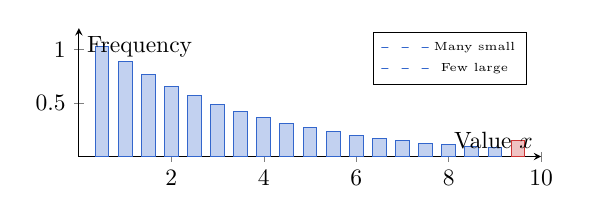
\begin{tikzpicture}[scale=0.85]
      \begin{axis}[
          width=0.7\textwidth, height=3.5cm,
          xmin=0, xmax=10, ymin=0, ymax=1.2,
          axis lines=middle,
          xlabel={Value $x$}, ylabel={Frequency},
          legend pos=north east,
          legend style={font=\tiny}
        ]
        % Many small bars, few large bars
        \foreach \x in {0.5,1,1.5,2,2.5,3,3.5,4,4.5,5,5.5,6,6.5,7,7.5,8,8.5,9,9.5}
          \addplot[datacolor, fill=datacolor!30, ybar, bar width=0.3] coordinates {(\x, {1.2*exp(-0.3*\x)})};
        \addplot[fitcolor, fill=fitcolor!30, ybar, bar width=0.3] coordinates {(9.5, 0.15)};
        \legend{Many small, Few large}
      \end{axis}
    \end{tikzpicture}
  \end{center}
  Power-laws describe scale-invariant phenomena: the ratio of frequencies is constant across scales.
\end{frame}

% --- Power-Law Formula and Properties ---
\begin{frame}{Power-Law Formula and Properties}
  \small
  \textbf{Mathematical form:} $P(x) = C \cdot x^{-\alpha}$ for $x \geq x_{\min}$.
  \vspace{0.2cm}
  \begin{itemize}
    \item $\alpha > 0$ is the power-law exponent (typically $1 < \alpha < 3$)
    \item \textbf{Lower $\alpha$} = heavier tail (more extreme values)
    \item \textbf{Higher $\alpha$} = lighter tail (more concentrated)
  \end{itemize}
  \vspace{0.2cm}
  \begin{center}
    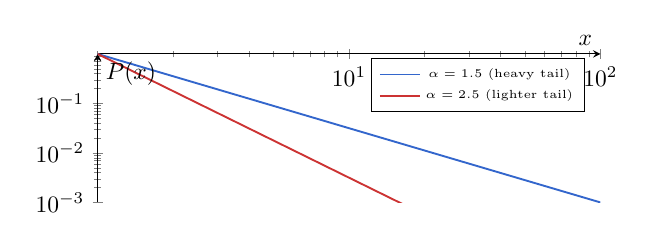
\begin{tikzpicture}[scale=0.85]
      \begin{axis}[
          width=0.75\textwidth, height=3.8cm,
          xmin=1, xmax=100, ymin=0.001, ymax=1,
          xmode=log, ymode=log,
          axis lines=middle,
          xlabel={$x$}, ylabel={$P(x)$},
          legend pos=north east,
          legend style={font=\tiny}
        ]
        \addplot[datacolor, thick, domain=1:100, samples=100] {x^(-1.5)};
        \addplot[fitcolor, thick, domain=1:100, samples=100] {x^(-2.5)};
        \legend{$\alpha=1.5$ (heavy tail), $\alpha=2.5$ (lighter tail)}
      \end{axis}
    \end{tikzpicture}
  \end{center}
  On log-log scale, both are straight lines with different slopes.
\end{frame}

% --- Why Log-Log Plots? ---
\begin{frame}{Why Log-Log Plots?}
  \small
  \textbf{Problem:} Power-laws span many orders of magnitude (hard to visualize on linear scale).
  \vspace{0.15cm}
  \textbf{Solution:} Take logarithm of both axes.
  \vspace{0.15cm}
  \textbf{Key insight:} $\log(P(x)) = \log(C) - \alpha \cdot \log(x)$
  \vspace{0.15cm}
  This is a \textbf{straight line}: $y = \text{intercept} - \alpha \cdot x$
  \vspace{0.2cm}
  \begin{columns}
    \column{0.48\textwidth}
    \begin{center}
      \textbf{Linear scale}\\[0.1cm]
      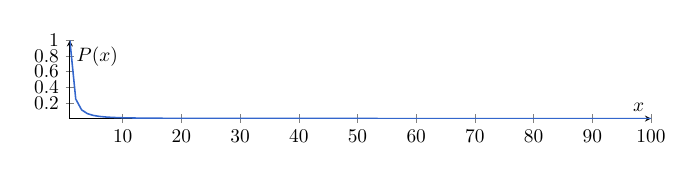
\begin{tikzpicture}[scale=0.7]
        \begin{axis}[
            width=\textwidth, height=3cm,
            xmin=1, xmax=100, ymin=0, ymax=1,
            axis lines=middle,
            xlabel={$x$}, ylabel={$P(x)$}
          ]
          \addplot[datacolor, thick, domain=1:100, samples=100] {x^(-2)};
        \end{axis}
      \end{tikzpicture}
      Hard to see pattern!
    \end{center}
    \column{0.48\textwidth}
    \begin{center}
      \textbf{Log-log scale}\\[0.1cm]
      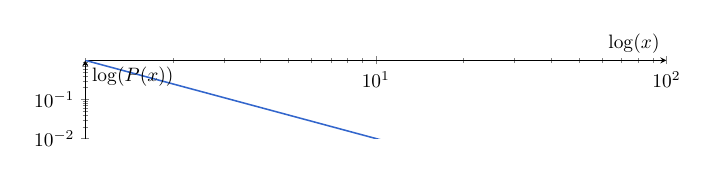
\begin{tikzpicture}[scale=0.7]
        \begin{axis}[
            width=\textwidth, height=3cm,
            xmin=1, xmax=100, ymin=0.01, ymax=1,
            xmode=log, ymode=log,
            axis lines=middle,
            xlabel={$\log(x)$}, ylabel={$\log(P(x))$}
          ]
          \addplot[datacolor, thick, domain=1:100, samples=100] {x^(-2)};
        \end{axis}
      \end{tikzpicture}
      Straight line!
    \end{center}
  \end{columns}
\end{frame}

% --- Log-Log Rank-Order Plots ---
\begin{frame}{Log-Log Rank-Order Plots}
  \small
  \textbf{Method:} Sort data from largest to smallest, then plot.
  \vspace{0.2cm}
  \begin{itemize}
    \item \textbf{X-axis:} $\log(\text{rank})$ where rank = 1, 2, 3, \ldots
    \item \textbf{Y-axis:} $\log(\text{value})$ for each ranked value
    \item If power-law: points form a \textbf{straight line}
    \item The \textbf{slope} $= -\alpha$ (negative of the power-law exponent)
  \end{itemize}
  \vspace{0.2cm}
  \begin{center}
    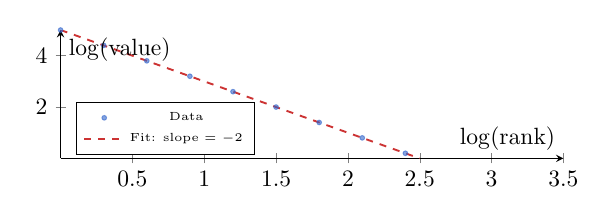
\begin{tikzpicture}[scale=0.85]
      \begin{axis}[
          width=0.75\textwidth, height=3.5cm,
          xmin=0, xmax=3.5, ymin=0, ymax=5,
          axis lines=middle,
          xlabel={$\log(\text{rank})$}, ylabel={$\log(\text{value})$},
          legend pos=south west,
          legend style={font=\tiny}
        ]
        % Simulated rank-order data (power-law with α=2) - points lie exactly on line y = 5.0 - 2*x
        \addplot[datacolor, only marks, mark=*, mark size=1pt, opacity=0.6] coordinates {
          (0,5.0) (0.3,4.4) (0.6,3.8) (0.9,3.2) (1.2,2.6) (1.5,2.0) (1.8,1.4) (2.1,0.8) (2.4,0.2)
        };
        % Fitted line: slope = -2
        \addplot[fitcolor, thick, dashed, domain=0:2.5] {5.0 - 2*x};
        \legend{Data, Fit: slope = $-2$}
      \end{axis}
    \end{tikzpicture}
  \end{center}
  Slope of fitted line gives the power-law exponent: $\alpha = -\text{slope}$.
\end{frame}

% --- Example 1: Clean Power-Law ---
\begin{frame}{Example 1: Clean Power-Law (Pareto Distribution)}
  \small
  Pareto distribution with $\alpha = 2.0$: $P(x) = C \cdot x^{-2}$ for $x \geq x_{\min}$.
  \vspace{0.2cm}
  \begin{center}
    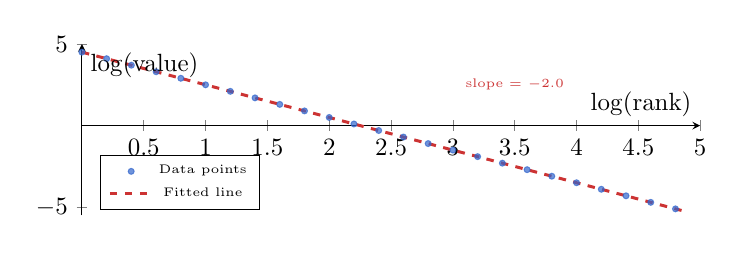
\begin{tikzpicture}[scale=0.9]
      \begin{axis}[
          width=0.85\textwidth, height=4cm,
          xmin=0, xmax=5, ymin=-5.5, ymax=5,
          axis lines=middle,
          xlabel={$\log(\text{rank})$}, ylabel={$\log(\text{value})$},
          legend pos=south west,
          legend style={font=\tiny}
        ]
        % Generate Pareto-like rank-order data (α=2 means slope=-2) - points on line y = 4.5 - 2*x
        \addplot[datacolor, only marks, mark=*, mark size=1.2pt, opacity=0.7] coordinates {
          (0,4.5) (0.2,4.1) (0.4,3.7) (0.6,3.3) (0.8,2.9) (1.0,2.5) (1.2,2.1) (1.4,1.7) (1.6,1.3) (1.8,0.9) (2.0,0.5) (2.2,0.1) (2.4,-0.3) (2.6,-0.7) (2.8,-1.1) (3.0,-1.5) (3.2,-1.9) (3.4,-2.3) (3.6,-2.7) (3.8,-3.1) (4.0,-3.5) (4.2,-3.9) (4.4,-4.3) (4.6,-4.7) (4.8,-5.1)
        };
        % Fitted line with slope -2.0
        \addplot[fitcolor, very thick, dashed, domain=0:4.9] {4.5 - 2.0*x};
        \node[fitcolor] at (3.5,2.5) {\tiny slope = $-2.0$};
        \legend{Data points, Fitted line}
      \end{axis}
    \end{tikzpicture}
  \end{center}
  \textbf{Result:} Slope $\approx -2.0$, so $\alpha \approx 2.0$ (matches theoretical value).
\end{frame}

% --- Inferring the Exponent ---
\begin{frame}{Inferring the Exponent}
  \small
  \textbf{Step-by-step process:}
  \vspace{0.2cm}
  \begin{enumerate}
    \item Create log-log rank-order plot (sort data, take logs)
    \item Fit a line (linear regression on log scale)
    \item Extract slope $m$
    \item Power-law exponent $\alpha = -m$
  \end{enumerate}
  \vspace{0.2cm}
  \textbf{Formula:} $\log(\text{value}) = \text{intercept} + m \cdot \log(\text{rank})$, so $\alpha = -m$.
  \vspace{0.3cm}
  \begin{center}
    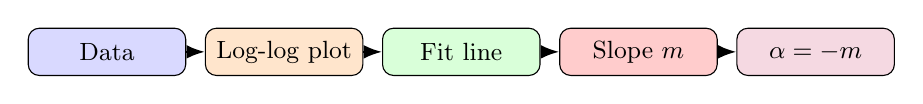
\begin{tikzpicture}[scale=0.9, every node/.style={font=\small}, box/.style={draw, rounded corners, minimum height=0.6cm, minimum width=2cm}, arrow/.style={-Latex, thick}]
      \node[box, fill=blue!15] (data) at (0,0) {Data};
      \node[box, fill=orange!20] (plot) at (2.5,0) {Log-log plot};
      \node[box, fill=green!15] (fit) at (5,0) {Fit line};
      \node[box, fill=red!20] (slope) at (7.5,0) {Slope $m$};
      \node[box, fill=purple!15] (alpha) at (10,0) {$\alpha = -m$};
      \draw[arrow] (data) -- (plot);
      \draw[arrow] (plot) -- (fit);
      \draw[arrow] (fit) -- (slope);
      \draw[arrow] (slope) -- (alpha);
    \end{tikzpicture}
  \end{center}
\end{frame}

% --- Power-Law vs Normal ---
\begin{frame}{Example 2: Power-Law vs Normal Distribution}
  \small
  Compare power-law (Pareto) vs normal distribution on log-log rank-order plots.
  \vspace{0.2cm}
  \begin{columns}
    \column{0.48\textwidth}
    \begin{center}
      \textbf{Power-Law}\\[0.1cm]
      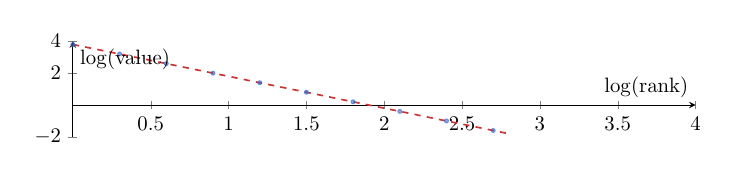
\begin{tikzpicture}[scale=0.75]
        \begin{axis}[
            width=\textwidth, height=3.2cm,
            xmin=0, xmax=4, ymin=-2, ymax=4,
            axis lines=middle,
            xlabel={$\log(\text{rank})$}, ylabel={$\log(\text{value})$}
          ]
          \addplot[datacolor, only marks, mark=*, mark size=1pt, opacity=0.6] coordinates {
            (0,3.8) (0.3,3.2) (0.6,2.6) (0.9,2.0) (1.2,1.4) (1.5,0.8) (1.8,0.2) (2.1,-0.4) (2.4,-1.0) (2.7,-1.6)
          };
          \addplot[fitcolor, thick, dashed, domain=0:2.8] {3.8 - 2*x};
        \end{axis}
      \end{tikzpicture}
      Straight line!
    \end{center}
    \column{0.48\textwidth}
    \begin{center}
      \textbf{Normal}\\[0.1cm]
      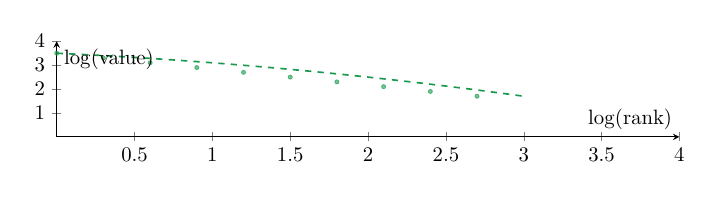
\begin{tikzpicture}[scale=0.75]
        \begin{axis}[
            width=\textwidth, height=3.2cm,
            xmin=0, xmax=4, ymin=0, ymax=4,
            axis lines=middle,
            xlabel={$\log(\text{rank})$}, ylabel={$\log(\text{value})$}
          ]
          \addplot[normalcolor, only marks, mark=*, mark size=1pt, opacity=0.6] coordinates {
            (0,3.5) (0.3,3.3) (0.6,3.1) (0.9,2.9) (1.2,2.7) (1.5,2.5) (1.8,2.3) (2.1,2.1) (2.4,1.9) (2.7,1.7)
          };
          \addplot[normalcolor, thick, dashed, domain=0:3] {3.5 - 0.3*x - 0.1*x^2};
        \end{axis}
      \end{tikzpicture}
      Curved (not power-law)
    \end{center}
  \end{columns}
  \vspace{0.2cm}
  Power-law: straight line on log-log plot. Normal: curved (exponential decay in tails).
\end{frame}

% --- Power-Law with Noise (Introduction) ---
\begin{frame}{Power-Law with Noise (Introduction)}
  \small
  \textbf{Real data is noisy!} Noise can obscure the power-law pattern.
  \vspace{0.2cm}
  \begin{itemize}
    \item Measurement errors, sampling variability, finite-size effects
    \item Still possible to detect and measure if noise is not too large
    \item Visual inspection and statistical tests help identify power-laws
  \end{itemize}
  \vspace{0.2cm}
  \begin{columns}
    \column{0.48\textwidth}
    \begin{center}
      \textbf{Clean}\\[0.1cm]
      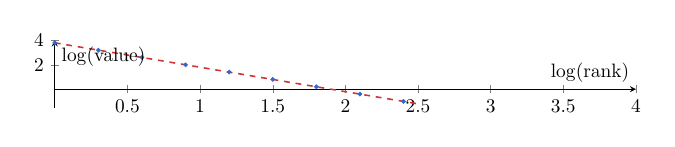
\begin{tikzpicture}[scale=0.7]
        \begin{axis}[
            width=\textwidth, height=2.8cm,
            xmin=0, xmax=4, ymin=-1.5, ymax=4,
            axis lines=middle,
            xlabel={$\log(\text{rank})$}, ylabel={$\log(\text{value})$}
          ]
          \addplot[datacolor, only marks, mark=*, mark size=1pt] coordinates {
            (0,3.8) (0.3,3.2) (0.6,2.6) (0.9,2.0) (1.2,1.4) (1.5,0.8) (1.8,0.2) (2.1,-0.4) (2.4,-1.0)
          };
          \addplot[fitcolor, thick, dashed, domain=0:2.5] {3.8 - 2*x};
        \end{axis}
      \end{tikzpicture}
    \end{center}
    \column{0.48\textwidth}
    \begin{center}
      \textbf{Noisy}\\[0.1cm]
      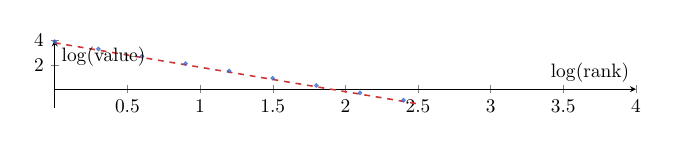
\begin{tikzpicture}[scale=0.7]
        \begin{axis}[
            width=\textwidth, height=2.8cm,
            xmin=0, xmax=4, ymin=-1.5, ymax=4,
            axis lines=middle,
            xlabel={$\log(\text{rank})$}, ylabel={$\log(\text{value})$}
          ]
          \addplot[datacolor, only marks, mark=*, mark size=1pt, opacity=0.7] coordinates {
            (0,3.9) (0.3,3.3) (0.6,2.7) (0.9,2.1) (1.2,1.5) (1.5,0.9) (1.8,0.3) (2.1,-0.3) (2.4,-0.9)
          };
          \addplot[fitcolor, thick, dashed, domain=0:2.5] {3.8 - 2*x};
        \end{axis}
      \end{tikzpicture}
    \end{center}
  \end{columns}
\end{frame}

% --- Noisy Power-Law (Low Noise) ---
\begin{frame}{Example 3: Noisy Power-Law (Low Noise)}
  \small
  Add small Gaussian noise to power-law data ($\alpha = 2.0$). Points scatter around the line but pattern is still visible.
  \vspace{0.2cm}
  \begin{center}
    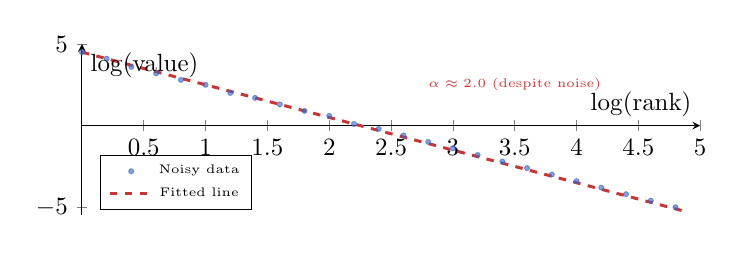
\begin{tikzpicture}[scale=0.9]
      \begin{axis}[
          width=0.85\textwidth, height=4cm,
          xmin=0, xmax=5, ymin=-5.5, ymax=5,
          axis lines=middle,
          xlabel={$\log(\text{rank})$}, ylabel={$\log(\text{value})$},
          legend pos=south west,
          legend style={font=\tiny}
        ]
        % Noisy power-law data (small noise) - base line y = 4.5 - 2*x with small random offsets
        \addplot[datacolor, only marks, mark=*, mark size=1pt, opacity=0.6] coordinates {
          (0,4.5) (0.2,4.1) (0.4,3.6) (0.6,3.2) (0.8,2.8) (1.0,2.5) (1.2,2.0) (1.4,1.7) (1.6,1.3) (1.8,0.9) (2.0,0.6) (2.2,0.1) (2.4,-0.2) (2.6,-0.6) (2.8,-1.0) (3.0,-1.4) (3.2,-1.8) (3.4,-2.2) (3.6,-2.6) (3.8,-3.0) (4.0,-3.4) (4.2,-3.8) (4.4,-4.2) (4.6,-4.6) (4.8,-5.0)
        };
        % Fitted line
        \addplot[fitcolor, very thick, dashed, domain=0:4.9] {4.5 - 2.0*x};
        \node[fitcolor] at (3.5,2.5) {\tiny $\alpha \approx 2.0$ (despite noise)};
        \legend{Noisy data, Fitted line}
      \end{axis}
    \end{tikzpicture}
  \end{center}
  \textbf{Result:} $\alpha$ can still be estimated reasonably well ($\alpha \approx 2.0$).
\end{frame}

% --- Noisy Power-Law (High Noise) ---
\begin{frame}{Example 4: Noisy Power-Law (High Noise)}
  \small
  Add larger Gaussian noise to power-law data. Points scatter more widely; still possible to fit, but less accurate.
  \vspace{0.2cm}
  \begin{center}
    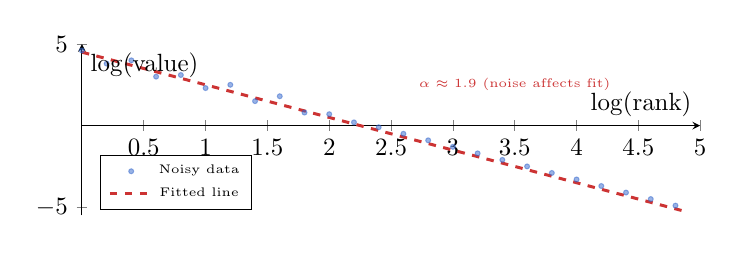
\begin{tikzpicture}[scale=0.9]
      \begin{axis}[
          width=0.85\textwidth, height=4cm,
          xmin=0, xmax=5, ymin=-5.5, ymax=5,
          axis lines=middle,
          xlabel={$\log(\text{rank})$}, ylabel={$\log(\text{value})$},
          legend pos=south west,
          legend style={font=\tiny}
        ]
        % High noise power-law data - base line y = 4.5 - 2*x with larger random offsets
        \addplot[datacolor, only marks, mark=*, mark size=1pt, opacity=0.5] coordinates {
          (0,4.6) (0.2,3.8) (0.4,4.0) (0.6,3.0) (0.8,3.1) (1.0,2.3) (1.2,2.5) (1.4,1.5) (1.6,1.8) (1.8,0.8) (2.0,0.7) (2.2,0.2) (2.4,-0.1) (2.6,-0.5) (2.8,-0.9) (3.0,-1.3) (3.2,-1.7) (3.4,-2.1) (3.6,-2.5) (3.8,-2.9) (4.0,-3.3) (4.2,-3.7) (4.4,-4.1) (4.6,-4.5) (4.8,-4.9)
        };
        % Fitted line (slightly off due to noise)
        \addplot[fitcolor, very thick, dashed, domain=0:4.9] {4.5 - 2.0*x};
        \node[fitcolor] at (3.5,2.5) {\tiny $\alpha \approx 1.9$ (noise affects fit)};
        \legend{Noisy data, Fitted line}
      \end{axis}
    \end{tikzpicture}
  \end{center}
  \textbf{Result:} Estimate is less accurate ($\alpha \approx 1.9$ vs true $2.0$); need more data or better methods.
\end{frame}

% --- Detecting Power-Laws in Noisy Data ---
\begin{frame}{Detecting Power-Laws in Noisy Data}
  \small
  \textbf{Methods:}
  \vspace{0.15cm}
  \begin{itemize}
    \item \textbf{Visual inspection:} Do points roughly follow a line?
    \item \textbf{Statistical test:} $R^2$ of linear fit on log scale
    \item \textbf{Threshold:} $R^2 > 0.9$ suggests power-law (adjust based on noise level)
    \item \textbf{Caution:} Noise can create false positives
  \end{itemize}
  \vspace{0.2cm}
  \begin{columns}
    \column{0.32\textwidth}
    \begin{center}
      \textbf{Clear}\\[0.1cm]
      \tiny $R^2 = 0.98$\\[0.1cm]
      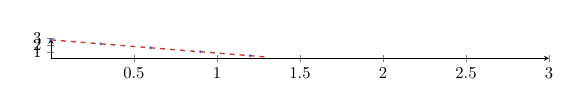
\begin{tikzpicture}[scale=0.6]
        \begin{axis}[width=\textwidth, height=2cm, xmin=0, xmax=3, ymin=0, ymax=3, axis lines=middle]
          \addplot[datacolor, only marks, mark=*, mark size=0.8pt, opacity=0.6] coordinates {(0,2.8) (0.3,2.2) (0.6,1.6) (0.9,1.0) (1.2,0.4)};
          \addplot[fitcolor, thick, dashed, domain=0:1.3] {2.8 - 2*x};
        \end{axis}
      \end{tikzpicture}
    \end{center}
    \column{0.32\textwidth}
    \begin{center}
      \textbf{Marginal}\\[0.1cm]
      \tiny $R^2 = 0.85$\\[0.1cm]
      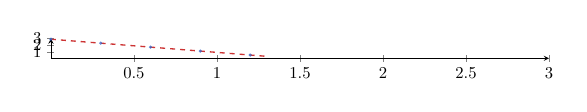
\begin{tikzpicture}[scale=0.6]
        \begin{axis}[width=\textwidth, height=2cm, xmin=0, xmax=3, ymin=0, ymax=3, axis lines=middle]
          \addplot[datacolor, only marks, mark=*, mark size=0.8pt, opacity=0.6] coordinates {(0,2.9) (0.3,2.3) (0.6,1.7) (0.9,1.1) (1.2,0.5)};
          \addplot[fitcolor, thick, dashed, domain=0:1.3] {2.9 - 2*x};
        \end{axis}
      \end{tikzpicture}
    \end{center}
    \column{0.32\textwidth}
    \begin{center}
      \textbf{Not power-law}\\[0.1cm]
      \tiny $R^2 = 0.45$\\[0.1cm]
      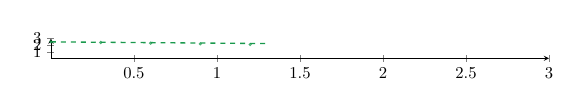
\begin{tikzpicture}[scale=0.6]
        \begin{axis}[width=\textwidth, height=2cm, xmin=0, xmax=3, ymin=0, ymax=3, axis lines=middle]
          \addplot[normalcolor, only marks, mark=*, mark size=0.8pt, opacity=0.6] coordinates {(0,2.5) (0.3,2.4) (0.6,2.3) (0.9,2.2) (1.2,2.1)};
          \addplot[normalcolor, thick, dashed, domain=0:1.3] {2.5 - 0.2*x};
        \end{axis}
      \end{tikzpicture}
    \end{center}
  \end{columns}
\end{frame}

% --- Real-World Example: City Sizes ---
\begin{frame}{Real-World Example: City Sizes}
  \small
  City population data often follows power-law (\textbf{Zipf's law}): rank $\times$ population $\approx$ constant.
  \vspace{0.2cm}
  \begin{itemize}
    \item Rank cities by population (largest = rank 1)
    \item Plot on log-log scale
    \item Typically $\alpha \approx 1.0$ (Zipf's law: $P(x) \propto x^{-1}$)
  \end{itemize}
  \vspace{0.2cm}
  \begin{center}
    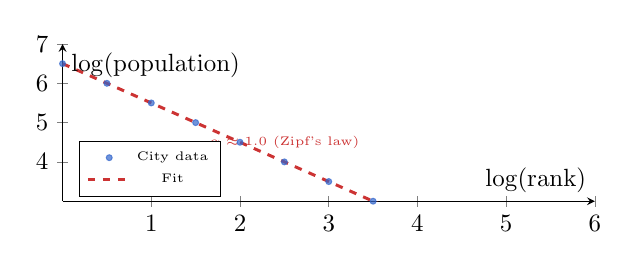
\begin{tikzpicture}[scale=0.9]
      \begin{axis}[
          width=0.75\textwidth, height=3.8cm,
          xmin=0, xmax=6, ymin=3, ymax=7,
          axis lines=middle,
          xlabel={$\log(\text{rank})$}, ylabel={$\log(\text{population})$},
          legend pos=south west,
          legend style={font=\tiny}
        ]
        % Stylized city size data (Zipf: α=1, so slope=-1) - points on line y = 6.5 - 1.0*x
        \addplot[datacolor, only marks, mark=*, mark size=1.2pt, opacity=0.7] coordinates {
          (0,6.5) (0.5,6.0) (1.0,5.5) (1.5,5.0) (2.0,4.5) (2.5,4.0) (3.0,3.5) (3.5,3.0)
        };
        \addplot[fitcolor, very thick, dashed, domain=0:3.6] {6.5 - 1.0*x};
        \node[fitcolor] at (2.5,4.5) {\tiny $\alpha \approx 1.0$ (Zipf's law)};
        \legend{City data, Fit}
      \end{axis}
    \end{tikzpicture}
  \end{center}
  Many other examples: word frequencies, network degrees, earthquake magnitudes, income distributions.
\end{frame}

% --- Recap ---
\begin{frame}{Recap}
  \small
  \begin{itemize}
    \item \textbf{Power-law:} $P(x) \propto x^{-\alpha}$ (many small values, few large values)
    \item \textbf{Log-log rank-order plots} reveal power-laws as straight lines
    \item \textbf{Slope of line} $= -\alpha$ (power-law exponent)
    \item \textbf{Noise} makes detection harder but still possible (use $R^2$ and visual inspection)
    \item \textbf{Common} in many natural and social phenomena: city sizes, word frequencies, networks, earthquakes
  \end{itemize}
  \vspace{0.3cm}
  \begin{center}
    \textbf{Key takeaway:} On log-log plots, power-laws appear as straight lines.\\
    The slope gives you the exponent: $\alpha = -\text{slope}$.
  \end{center}
\end{frame}

\end{document}
